\documentclass{report}
\usepackage{polski}
\usepackage[utf8]{inputenc}
\usepackage{float}
\usepackage{graphicx}
\usepackage{caption}
\usepackage{subcaption}
\usepackage{ragged2e}
\usepackage{blindtext}
\usepackage{hyperref}
\usepackage{listings}
\usepackage{color}

\definecolor{dkgreen}{rgb}{0,0.6,0}
\definecolor{gray}{rgb}{0.5,0.5,0.5}
\definecolor{mauve}{rgb}{0.58,0,0.82}

\lstset{
  language=SQL,
  aboveskip=3mm,
  belowskip=3mm,
  showstringspaces=false,
  columns=flexible,
  basicstyle={\small\ttfamily},
  numbers=none,
  numberstyle=\tiny\color{gray},
  keywordstyle=\color{blue},
  commentstyle=\color{dkgreen},
  stringstyle=\color{mauve},
  breaklines=true,
  breakatwhitespace=true,
  tabsize=3
}

\begin{document}
\title{Project - Eatter}
\author{Jakub Ogrodowczyk}
\author{Dawid Walczak}
%\AddToHook{cmd/section/before}{\clearpage}

\section*{Ogólny zarys projektu}
Jako nasz projekt postanowiliśmy stworzyć platformę Social Media
skupiającą się na ocenianiu zjedzonych posiłków w restauracjach.
Poniżej widać projekt naszej bazy danych:

\begin{figure}[h]
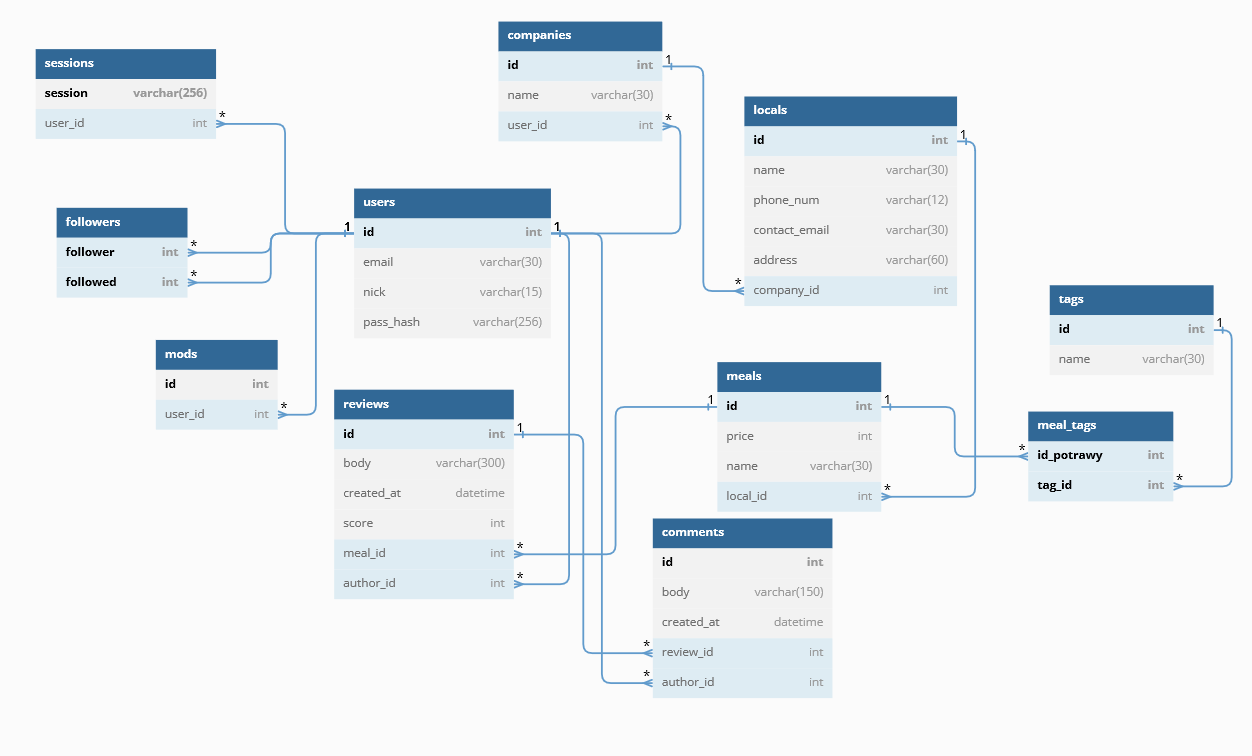
\includegraphics[width=\textwidth]{./diagram.png}
\caption[Example .]{Diagram projektu bazy danych}
\end{figure}

\section*{Założenia związane z poziomami dostępu}
Na platformie przewidziane były cztery różne poziomy dostępu:
\begin{enumerate}
    \item Niezalogowany użytkownik
    \item Zalogowany użytkownik
    \item Właściciel restauracji
    \item Moderator
\end{enumerate}
\subsection*{Niezalogowany użytkownik}
Osoba niezalogowana ma możliwość przeglądania recenzji, wyszukiwania
konkretnego dania po nazwie lub tagach, utworzenia konta
oraz samej czynności zalogowania.
Ponadto na tym etapie również sprawdzana jest poprawność danych przy
logowaniu.
\subsection*{Zalogowany użytkownik}
Gdy użytkownik już się zaloguje tworzona jest \textbf{sesja}. W tabeli
\textbf{sessions} tworzymy nowy rekord łączący token sesji z ID użytkownika.
Analogicznie, przy wylogowywaniu (lub po upłynięciu pewnej ilości czasu)
sesja będzie usuwana z tabeli. Token sesji potrzebny od strony clienta do
tworzenia zapytań, ponieważ nie przechowujemy we frontendzie ID użytkownika.
Ponadto zalogowany użytkownik ma dostęp do swojego profilu, personalną tablicę
składającą się z postów użytkowników, których obserwuje oraz możliwość komentowania
i dodawania postów.
\subsection*{Właściciel restauracji}
Właściciel restauracji jest rozszerzeniem funkcjonalności użytkownika. Ma on
dodatkowo dostęp do dodawania i moderowania dań w swoich restauracjach.
\subsection*{Moderator}
Moderator również jest rozszerzeniem funkcjonalności użytkownika. Może on
usuwać i modyfikować posty, a także i konta użytkowników.

\section*{Normalizacja}

\subsection*{1 NF}
Baza danych znajduje się w pierwszej formie normalnej. 
W każdej tabeli znajduje się klucz główny unikalny służący do rozróżniania krotek.
Także każdy atrybut to jedna atomowa wartość - liczba, data lub tekst.
Do zapewnienia tego zostały utworzone odpowiednie tabele relacji wiele do wielu, takie jak 
\textbf{followers} i \textbf{meals\_tags}.


\subsection*{2 NF}
Dodatkowo spełniona jest druga forma normalna. 
W każdej tabeli atrybuty niekluczowe zależą jedynie od pełnego klucza.
Na przykład w tabeli \textbf{locals}. Wszystkie atrybuty są właściwością 
konkretnego lokalu. Atrybuty, które takie nie były, na przykład informacje
o firmie zarządzającej obiektem, zostały przeniesione do osobnej tabeli \textbf{companies}
i powiązane z tą przez klucz obcy.
\begin{center}
\begin{tabular}{|c|}
    \hline
    \textbf{locals} \\
    \hline \hline
    \textbf{id} \\
    \hline
    name \\
    \hline
    phone\_num \\
    \hline
    contact\_email \\
    \hline
    address \\
    \hline
    company\_id \\
    \hline
\end{tabular}
\end{center}

\subsection*{3 NF}
Trzecia forma normalna także jest spełniona. We wszystkich tabelach,
wszystkie atrybuty niekluczowe zależą jedynie od klucza głównego.

\section*{Szczegółowe omówienie tabel}
\subsection*{Users}
Tabela użytkowników zgodnie z nazwą zawiera wszystkie informacje
powiązane z kontem danego użytkownika. Do zalogowania użytkownik
musi podać swój email i hasło - dlatego email jest wartością
unikalną. W bazie przechowujemy tylko i wyłącznie hash hasła,
które hashowane są na backendzie przy pomocy funkcji \textbf{Argon2}.
\begin{lstlisting}[language=SQL]
    CREATE TABLE users (
        id int NOT NULL AUTO_INCREMENT,
        email varchar(30) NOT NULL UNIQUE, 
        nick varchar(15) NOT NULL,
        pass_hash varchar(256) NOT NULL,
        PRIMARY KEY (id)
    );
\end{lstlisting}

\subsection*{Mods}
Tak jak było wyżej wspomniane, moderator jest rozszerzeniem nad
użytkownikiem. Z punktu widzenia bazy, ta tabela nie zawiera żadnych
dodatkowych danych (poza unikalnym ID), a jest jedynie oznaczeniem
poszczególnych kont jako posiadających uprawnienia moderatora.
\begin{lstlisting}[language=SQL]
    CREATE TABLE mods (
        id int NOT NULL AUTO_INCREMENT, 
        user_id int NOT NULL,
        PRIMARY KEY (id),
        FOREIGN KEY (user_id) REFERENCES users(id)
    );
\end{lstlisting}

\subsection*{Followers}
W tej tabeli łączymy użytkowników w pary (follower, followed).
Używamy jej później przy filtrowaniu postów na tablicy.
\begin{lstlisting}[language=SQL]
    CREATE TABLE followers (
        follower int NOT NULL, 
        followed int NOT NULL, 
        PRIMARY KEY (follower, followed),
        FOREIGN KEY (follower) REFERENCES users(id),
        FOREIGN KEY (followed) REFERENCES users(id)
    );
\end{lstlisting}


\subsection*{Companies}
Firma w naszej bazie jest, podobnie jak moderator, rozszerzeniem
nad użytkownikiem. Z punktu widzenia bazy, rozszerza ona go tylko o
unikalną nazwę firmy. Firma nie jest natomiast konkretną placówką,
a raczej reprezentacją właściciela owej placówki w naszej bazie.
Jako firmę zapisujemy jednocześnie sieciówki, takie jak przykładowo
MCDonald's, ale też i prywatnych właścicieli posiadających jedną
restuarację.
\begin{lstlisting}[language=SQL]
    CREATE TABLE companies ( 
        id int NOT NULL AUTO_INCREMENT,
        name varchar(30) NOT NULL UNIQUE,
        user_id int NOT NULL UNIQUE,
        PRIMARY KEY (id),
        FOREIGN KEY (user_id) REFERENCES users(id)
    );
\end{lstlisting}

\subsection*{Locals}
Lokal reprezentuje konkretną placówkę należącą do danej firmy
z tabeli \textbf{Companies}. Zawiera on w sobie wszystkie dane konieczne
do ewentualnego skontaktowania lub odnalezienia restauracji.
\begin{lstlisting}[language=SQL]
    CREATE TABLE locals (
        id int NOT NULL AUTO_INCREMENT,
        name varchar(30) NOT NULL,
        phone_num varchar(12) NOT NULL,
        contact_email varchar(30) NOT NULL,
        address varchar(60) NOT NULL,
        company_id int NOT NULL,
        PRIMARY KEY (id),
        FOREIGN KEY (company_id) REFERENCES companies(id)
    );
\end{lstlisting}

\subsection*{Meals}
Encja posiłku reprezentuje danie podawane w jakimś lokalu.
Ta tabela stoi oczywiście w samym sercu naszej aplikacji gdyż
jej głównym celem jest znajdowanie nowych smaków oraz dzielenie
się opinią na temat zjedzonych już potraw.
\begin{lstlisting}[language=SQL]
    CREATE TABLE meals (
        id int NOT NULL AUTO_INCREMENT,
        price FLOAT NOT NULL,
        name varchar(30) NOT NULL, 
        local_id int NOT NULL,
        PRIMARY KEY (id),
        FOREIGN KEY (local_id) REFERENCES locals(id)
    );
\end{lstlisting}

\subsection*{Tags}
Tagi używane są przy wyszukiwaniu. Nowe rekordy są tworzone
za każdym razem gdy ktoś dodaje do dania tag, który poprzednio
nie istniał.
\begin{lstlisting}[language=SQL]
    CREATE TABLE tags (
        id int NOT NULL AUTO_INCREMENT, 
        name varchar(30) NOT NULL UNIQUE,
        PRIMARY KEY (id)
    );
\end{lstlisting}

\subsection*{Meals\_Tags}
Tutaj łączymy poszczególne tagi do konkretnych posiłków.
Do tej tabeli dodany jest trigger, który dodaje do tabeli \textbf{Tags}
nowy rekord, jeśli próbujemy do dania dołożyć tag, który jeszcze nie istnieje.
Dodawane są one przez użytkowników z uprawnieniami \textbf{Companies}.
\begin{lstlisting}[language=SQL]
    CREATE TABLE meals_tags ( 
        meal_id int NOT NULL,
        tag_id int NOT NULL,
        PRIMARY KEY (meal_id, tag_id)
    );
\end{lstlisting}

\subsection*{Reviews}
Recenzja w naszej aplikacji jest równoznaczna z postem w tradycyjnym
modelu social media. Zawiera ona wszystkie dane potrzebne do
wyświetlenia jej na cliencie oraz zewnętrzne klucze łączące ją
z konkretnym użytkownikiem (autorem) oraz posiłkiem, którego ona dotyczy.
\begin{lstlisting}[language=SQL]
    CREATE TABLE reviews (
        id int NOT NULL AUTO_INCREMENT,
        body varchar(300) NOT NULL, 
        created_at datetime NOT NULL, 
        score int NOT NULL, 
        meal_id int NOT NULL, 
        author_id int NOT NULL,
        PRIMARY KEY (id),
        FOREIGN KEY (meal_id) REFERENCES meals(id),
        FOREIGN KEY (author_id) REFERENCES users(id)
    );
\end{lstlisting}

\subsection*{Comments}
Komentarze, w gruncie rzeczy, są podobną strukturą do obiektu recenzji.
Zamiast posiłku, do którego się odwołują, mają one ID recenzji.
\begin{lstlisting}[language=SQL]
    CREATE TABLE comments (
        id int NOT NULL AUTO_INCREMENT, 
        body varchar(150) NOT NULL, 
        created_at datetime NOT NULL, 
        review_id int NOT NULL, 
        author_id int NOT NULL,
        PRIMARY KEY (id),
        FOREIGN KEY (review_id) REFERENCES reviews(id),
        FOREIGN KEY (author_id) REFERENCES users(id)
    );
\end{lstlisting}

\subsection*{Sessions}
Tabela przechowująca obecnie otwarte sesje służy do bezpieczniejszej
komunikacji między clientem, a serverem. Nie tylko client nie musi teraz
przechowywać takich rzeczy jak ID usera, ale również rozwiązuje ona nam
problem implementacyjny frontendy związany z traceniem stanu aplikacji
przy przechodzeniu na różne podstrony. 
\begin{lstlisting}[language=SQL]
    CREATE TABLE sessions (
        session varchar(256) NOT NULL,
        user_id int NOT NULL,
        PRIMARY KEY (session),
        FOREIGN KEY (user_id) REFERENCES users(id)
    );
\end{lstlisting}

\section*{Komunikacja bazy z serwerem}
Serwer łączy się z bazą z poziomu użytkownika 'server'.
\begin{lstlisting}[language=SQL]
CREATE USER 'server'@'localhost' IDENTIFIED BY 'server';
SET PASSWORD FOR 'server'@'localhost' = PASSWORD('<enter_pass>');
GRANT EXECUTE ON eatter.* TO 'server'@'localhost';
\end{lstlisting}
Przyznajemy mu na razie tylko możliwość wchodzenia w interakcje z danymi
za pomocą procedur. Dzięki temu minimalizujemy ryzyko wypłynięcia lub
przypadkowego skasowania danych. Procedur tych jest cała masa, a tworzone
są głównie z myślą o konkretnych funkcjach istniejących już na backendzie.
Przykładem ciekawszych procedur, które można znaleźć w naszym projekcie
jest system obsługiwania loginów i sesji.
\begin{lstlisting}[language=SQL]
    DELIMITER //
    CREATE PROCEDURE createSession(IN user_id int)
    BEGIN
        IF NOT EXISTS (SELECT * FROM sessions WHERE sessions.user_id = user_id) THEN
            INSERT INTO sessions(session, user_id) VALUES (SHA2(user_id, 256), user_id);
        END IF;
        SELECT sessions.session FROM sessions WHERE sessions.user_id = user_id;
    END//

    CREATE FUNCTION verifyUser(email varchar(30), pass_hash varchar(256))
    RETURNS int
    BEGIN
        DECLARE user_id INT DEFAULT -1;
        SET user_id = (SELECT users.id FROM users WHERE users.email = email AND users.pass_hash = pass_hash);
        RETURN user_id;
    END//

    CREATE PROCEDURE loginUser(IN email varchar(30), IN pass_hash varchar(256))
    BEGIN
        DECLARE user_id INT;
        SET user_id = verifyUser(email, pass_hash);
        IF (user_id > -1) THEN
            CALL createSession(user_id);
        END IF;
    END//
    DELIMITER ;
\end{lstlisting}
Trzymanie timerów usuwających martwe sesje znajduje się już po stronie
serwera.
\section*{Optymalizacje}
\subsection*{Redundantne dane}
Użytkownik ma możliwość zobaczenia agregowanych danych 
na temat posiłków i lokali. W celu usprawnienia bazy danych,
zdenormalizowaliśmy bazę danych, dodając tabele z 
redundantnymi agregowanymi atrybutami, m. in. liczba recenzji
i średnia z ocen. Spójność jest kontrolowana przez odpowiednie triggery.

\section*{Technologie}
Aplikacja została stworzona przy pomocy standardowych technologii webowych.
Jako frontend korzystamy z frameworka \emph{Sveltekit}, który odpowiada za 
renderowanie serwerowe. Backend został zaimplementowany w języku
\emph{Rust} przy pomocy biblioteki \emph{Axum}, co pozwala na bezpieczeństwo
i wydajność. Baza danych to \emph{MariaDB}.

\end{document}

